The analysis follows the same strategy one used in 2016 p-Pb and pp data samples (see published paper \cite{ALICEDhcorr} and analysis notes \cite{Notepp}, \cite{NotepPb}). Correlation pairs are formed by
trigger particles (D mesons) reconstructed and selected in the following $\pt^{\rm trig}$ ranges: $3<\pt^{\rm trig}<5$ $\gev/c$, $5<\pt^{\rm trig}<8$ $\gev/c$, $8<\pt^{\rm trig}<16$ $\gev/c$, $16<\pt^{\rm trig}<24$ $\gev/c$ (the possibility of extending the analysis in $2<\pt^{\rm trig}<3$ was also exploited. Further details are furnished in the next paragraph). Associated particles (charged tracks) have been reconstructed in the following $\pt^{\rm assoc}$ regions: $\pt^{\rm assoc}>0.3$ $\gev/c$, $0.3<\pt^{\rm assoc}<1$ $\gev/c$, $1<\pt^{\rm assoc}<2$ $\gev/c$, $2<\pt^{\rm assoc}<3$ $\gev/c$, $\pt^{\rm assoc}>1$ $\gev/c$. In this analysis, the particle identification defines the trigger particle rather than a momentum cut and therefore the momentum range of the associated particles is not constrained by that of the trigger particle. Our definition of associated particle includes primary particles of the following species: pion, kaon, proton, electron, muon. The primary particle definition comprises particle coming from the primary vertex of interaction, including those coming from strong and electromagnetic decay of unstable particles, and particles deriving from the decay of hadrons with charm or beauty.
We therefore include any charged $\pi$,K,p,e,$\mu$ except those coming from weak decays of strange particles and particles produced in the interaction with the detector material. This definition corresponds to that used in the method AliAODMCParticle::IsPyhysicalPrimary().
All associated particles surviving the selection cuts and not matching the adopted criterion are considered as a contamination whose contribution has to be corrected for. \\

The analysis is performed through the following steps:

\begin{enumerate}
\item
\underline {\bf D meson selection and signal extraction.}  For each single event, ``trigger" particles
are defined as the selected  D meson candidates ($\Dzero$, $\Dplus$ and $\Dstar$)
within a given $\pt^{\rm trig}$ range. The detection strategy for D mesons at central rapidity is
the same performed for the analyses of the D-meson production at central rapidity~\cite{ALICEDmespp7Tev}, and also applied for the D-h analysis on 2016 pp and 2016 p-Pb samples (\cite{Notepp}, \cite{NotepPb}). It is based on the reconstruction of decay
vertices displayed from the primary vertex by a few hundred $\mu$m and on the identification of the decay-particle species.
The identification of the charged kaon and pion in the TPC and TOF detectors is also used, to further reduce the background at low $\pt$.  An invariant-mass analysis is then used to extract the raw signal yield, using the same fit functions described in~\cite{ALICEDhcorr}.
The D mesons are selected in the rapidity range varying from $|y|<0.5$ at low $\pt$ to $|y|<0.8$ for $\pt>5~\gev/c$. %The final results are corrected to have D mesons within $|y|<0.5$.

\item
\underline{\bf Correlation of D candidates with associated tracks.}
Particle pairs are formed by correlating each trigger particle with the charged primary particles passing the track selection (excluding those coming from the decay of the D-meson candidate) in a specified $p^{assoc}_{T}$ interval (which can overlap with the $\pt^{\rm trig}$ range) and in the pseudo-rapidity range $|\eta|<0.8$. For the $\Dzero$ meson, also the low-momentum pion tracks from feed-down of $\Dstar$ mesons are removed via 3$\sigma$ invariant mass cut on the $M(K\pi\pi)-M(K\pi)$ difference. This because these soft pion are not related to the charm quark fragmentation chain.
For D meson candidates in the invariant mass signal region, defined by a $\pm$ 2$\sigma$ interval around the D meson mass peak, the azimuthal angle difference $\varphi^{\rm assoc}-\varphi^{\rm trigg}\equiv\Delta\varphi$
and the pseudorapidity difference $\eta^{\rm assoc}-\eta^{\rm trig}\equiv\Delta \eta$ are evaluated and stored to build two-dimensional correlation distribution. % in a multi-dimensional histogram.

\item
\underline{\bf Correction for limited acceptance and detector inhomogeneities with Event Mixing}
The angular correlation distribution may be affected, even for uncorrelated pair of particles, by structures not due to physical effects, but originating from the limited detector acceptance, as well as from angular inhomogeneities in the trigger and track reconstruction efficiencies as a function of $\Delta\varphi$ and $\Delta\eta$.
Effects of this kind are removed using the Event Mixing technique.
In this technique, the analysis is executed on the same data sample of the standard one (called ``same event" analysis, SE), but the trigger particles found in each event are correlated to charged particles reconstructed in different events (``Mixed Events'' analysis, ME) with similar characteristic, in particular concerning the event multiplicity and z position of the primary vertex (see Section \ref{MEsection}). \\

The differential yield of associated particles per trigger particle is obtained by
\begin{linenomath}
  \begin{equation}
    \label{2pcorr_incl}
    \frac{1}{N_\text{trig}}\frac{\d^{2}N^\text{pair}}{\d\Delta\eta\, \d\Delta\varphi}
= B_{ME}(0,0)\times\frac{S(\Delta\eta,\Delta\varphi)}{B_{ME}(\Delta\eta,\Delta\varphi)},
\end{equation}
\end{linenomath}
where $N^\text{pair}$ is the total number of correlated D-hadron
pairs. The functions $S(\Delta\eta,\Delta\varphi)$ and
$B_{ME}(\Delta\eta,\Delta\varphi)$ are the signal and the mixed event
background distributions, respectively. The later is normalized to its value in
$(\Delta\eta,\Delta\varphi)=(0,0)$, i.e. ($B(0,0)$).
Further details on the mixed-event correction are provided in the next section.

\item
\underline{\bf Subtraction of background correlation from signal distribution.}
The invariant mass signal region also includes background D-meson candidates. Their contribution to the
raw correlation distribution is subtracted as follows. For each $\pt$ bin, the mean and the sigma of the
invariant mass spectrum are extracted. For $\Dzero$ and $\Dplus$, a ``background'' region is defined in the sidebands of the mass
distribution as the interval $4 ~ \gev/c^2<|m-m^{\rm pdg}|<8 ~ \gev/c^2$ (for the $\Dstar$ meson, only the right sideband is used). The angular correlation distribution for background candidates in this region is extracted and normalized with respect to the background in the signal region estimated from the mass fit. This normalized background correlation distribution is then subtracted from the
raw signal one to obtain the signal correlation distribution. The normalization factor is the ratio of the number of background candidates under the signal peak (obtained by integrating the background of the fit function within the signal region) over the number of background candidates in the sidebands (obtained via bin-counting in the sideband region).
An example of the signal region, sideband and sideband-subtracted 1D correlation distributions (along $\Delta\varphi$) is shown in figure \ref{signReg}, together with the comparison of the three distributions after the normalization to the number of triggers.

\begin{figure}[h]
\centering
\includegraphics[width=1\linewidth]{{figures/DStar_pp/h1D_Dstar_Canvas_PtIntBins7to9_PoolInt_thr0dot3to99dot0.png}}
\includegraphics[width=0.8\linewidth]{{figures/DStar_pp/h1D_Dstar_Canvas_Normalized_PtIntBins7to9_PoolInt_thr0dot3to99dot0}}
\caption{Top: Example of $\Dstar$-h signal region (left), sideband (middle), and signal minus sideband (right) correlation distributions. Bottom: signal region per-trigger normalized correlation distribution (blue), sideband region per-trigger normalized correlation distribution (red),
background-subtracted per-trigger normalized correlation distribution (black).}
\label{signReg}
\end{figure}

\item
\underline{\bf Correction for D meson efficiency and associated track efficiency.}
After filling the signal and background correlation distributions, it is necessary to take into account also for the correlations with tracks, those are not reconstructed, or not passing the quality selection due to poor reconstruction. In the same way, the loss of D-mesons which are not reconstructed, or do not pass the selection, impacts the correlation distribution shape. Hence, each pair is weighted by the inverse of the product of the associated track and D meson reconstruction efficiency, $\epsilon_{trk}$ and $\epsilon_{trig}$. Further details are provided later on in this section.

\item
\underline{\bf Projection in $\Delta\varphi$.}
The limited statistics available does not allow to study the two dimensional
$(\Delta\eta,\Delta\varphi)$ distribution, which is therefore projected to the $\Delta\varphi$ axis by integrating on $|\Delta\eta| <$ 1. Despite, in principle, our maximum $\Delta\eta$ acceptance is of $|\Delta\eta| <$ 1.6, removing the large $|\Delta\eta|$ regions allow us to reject angular regions with very low statistics, where fluctuations would be amplified by a large mixed-event correction, and avoid the so-called wings effect.

As the difference in the azimuthal angle is periodic ($\Delta \varphi = 0 = 2\pi$), the $\Delta\varphi$-range is limited to the essential range of 2$\pi$. The $\Delta \varphi$-limits are chosen to be [$-\pi$/2, 3$\pi$/2] in order to provide a good visibility of the correlation pattern, which peaks around 0 and $\pi$.

\item
\underline{\bf Correction for the contamination of secondary particles}
The DCA to primary vertex cut, applied during the associated track selection, has the role of removing the secondary particles from the associated track sample.
Secondary particles are indeed produced either from long-lived strange hadrons or from interaction of particles with the detector material. A residual contamination from secondary tracks is hence expected in the correlation distributions. This contamination is estimated from Monte Carlo simulation based on Pythia as described more in detail in the next section. The background-subtracted
event-mixing corrected correlations are multiplied by a purity factor to encounter this contribution.

\item
\underline{\bf Correction for bias on B to D decay topologies}
The presence of the topological cuts for the D-meson selection indirecly induce a bias on the topology of the B to D decay topologies, favouring cases with a small opening angle between the D-meson and the other tracks from the B decay. This affects the feed-down component of the data correlation distributions. This effect is corrected for with a procedure described in the subsection \ref{MCclosure}. %Note that this correction is a novelty with respect to the previous analyses, where only a quite conservative systematic uncertainty was applied to take into account this effect.

\item
\underline{\bf Correction for feed-down of D meson from b-hadron decay}
The selection strategy employed for the D meson candidates selection %to increase the signal over the combinatorial background
enhances the fraction of reconstructed D mesons coming from the decay of a b-hadron. Typical values, with the cuts used for the D-meson selection, are of the order of 10\% or less. The correlation distribution of these secondary D mesons will be sensitive to the properties of beauty jets and beauty hadron decay, which in general differ from those relative to charm jets and hadrons. The procedure used to subtract this contribution is described in the next paragraphs of this section.

\item
\underline{\bf Study of correlation properties.}
The properties of the azimuthal correlation distribution are quantified by fitting the distribution with a function composed of two Gaussian functions, modelling the near and the away side peaks, and a constant term describing the baseline. The mean of the Gaussian are fixed at $\Delta\varphi = 0$ and $\Delta\varphi = \pi$. To accomplish the $2\pi$ periodicity of the $\Delta\varphi$ variable, the Gaussian functions are ``duplicated'' with mean at $\Delta\varphi = 2\pi$ and $\Delta\varphi = -\pi$.
The fitting procedure is described in details in Section \ref{results}.


%The integral of the near side peak and the away side peak
%is dominated by the central parts of the peaks at
%$\Delta \varphi = 0$ and $\Delta \varphi = \pi$, respectively. Thus, minor
%shape deviations at the side of the peak regions are  acceptable. In
%the following, the fit function is introduced step by step.
%The $\Delta \varphi$ distribution can roughly be approximated by a
%constant and two Gaussian functions with the periodicity condition.
%As the $\Delta \varphi$-distribution is a periodically continuing
%distribution with $\Delta\varphi = 0 = 2\pi$, the fit function has to
%be periodically continuing as well.

\end{enumerate}

\subsection{Mass plots and cut optimization}
The invariant mass distributions of $\Dzero$, $\Dstar$ and $\Dplus$ in the various $\text{p}_T$ ranges are shown in Figure~\ref{fig:InvMassD0},~\ref{fig:InvMassDs} and~\ref{fig:InvMassDp} respectively. Note that the distributions are weighted by the D-meson selection and reconstruction efficiency, to allow a correct normalization of the correlation distributions, which have also these weights.

\begin{figure}[!htp]
\centering
{\includegraphics[width=0.94\textwidth]{figures/Dzero/InvMassDistributions_Dzero_Bins4to5.png}}
{\includegraphics[width=0.94\textwidth]{figures/Dzero/InvMassDistributions_Dzero_Bins6to8.png}}
\end{figure}
\begin{figure}[!htp]
\centering
{\includegraphics[width=0.94\textwidth]{figures/Dzero/InvMassDistributions_Dzero_Bins9to11.png}}
{\includegraphics[width=0.94\textwidth]{figures/Dzero/InvMassDistributions_Dzero_Bins12to13.png}}

%[width=.32\linewidth]
\caption{Invariant mass distributions of $D^0$ corrected with efficiency in different $\text{p}_T$ regions. Top: $3< p_{T}^{\text{D}}< 4$ $\gev/c$ (left), $4< p_{T}^{\text{D}}< 5$ $\gev/c$ right), Mid 1: $5< p_{T}^{\text{D}}< 6$ $\gev/c$ (left), $6 < p_{T}^{\text{D}} < 7$ $\gev/c$ (middle), $7< p_{T}^{\text{D}}< 8$ $\gev/c$ (right); Mid2: $8< p_{T}^{\text{D}}< 10$ $\gev/c$, $10< p_{T}^{\text{D}}< 12$ $\gev/c$  (middle), $12 < p_{T}^{\text{D}}< 16$ $\gev/c$  (right) and Bottom: $16<p_{T}^{\text{D}}< 24$ $\gev/c$.}
\label{fig:InvMassD0}
\end{figure}

\begin{figure}[!htp]
\centering
{\includegraphics[width=1\linewidth, height=5.6cm]{figures/DStar_pp/InvMassDistributions_Dstar_Bins2to3.png}}
{\includegraphics[width=1\linewidth, height=5.6cm]{figures/DStar_pp/InvMassDistributions_Dstar_Bins4to6.png}}
{\includegraphics[width=1\linewidth, height=5.6cm]{figures/DStar_pp/InvMassDistributions_Dstar_Bins7to9.png}}
{\includegraphics[width=0.6\linewidth, height=5.6cm]{figures/DStar_pp/InvMassDistributions_Dstar_Bins10to10.png}}

\caption{Invariant mass distributions of $\Dstar$ corrected with efficiency in different $\text{p}_T$ regions. Top: $3< p_{T}^{\text{D}}< 4$ $\gev/c$ (left), $4< p_{T}^{\text{D}}< 5$ $\gev/c$ right), Mid 1: $5< p_{T}^{\text{D}}< 6$ $\gev/c$ (left), $6 < p_{T}^{\text{D}} < 7$ $\gev/c$ (middle), $7< p_{T}^{\text{D}}< 8$ $\gev/c$ (right); Mid2: $8< p_{T}^{\text{D}}< 10$ $\gev/c$, $10< p_{T}^{\text{D}}< 12$ $\gev/c$  (middle), $12 < p_{T}^{\text{D}}< 16$ $\gev/c$  (right) and Bottom: $16<p_{T}^{\text{D}}< 24$ $\gev/c$ .}
\label{fig:InvMassDs}
\end{figure}

\begin{figure}[h]
\centering
{\includegraphics[width=0.94\textwidth]{figures/DplusPlotsweff/InvMassDistributions_Dplus_Bins3to4.png}}
{\includegraphics[width=0.94\textwidth]{figures/DplusPlotsweff/InvMassDistributions_Dplus_Bins5to7.png}}
\end{figure}

\begin{figure}[h]
\centering
{\includegraphics[width=0.94\textwidth]{figures/DplusPlotsweff/InvMassDistributions_Dplus_Bins8to12.png}}
{\includegraphics[width=0.94\textwidth]{figures/DplusPlotsweff/InvMassDistributions_Dplus_Bins13to13.png}}
\caption{Invariant mass distribution of $\Dplus$ corrected with efficiency in different $\text{p}_T$ regions. Top: $3< p_{T}^{\text{D}}< 4$ $\gev/c$ (left), $4< p_{T}^{\text{D}}< 5$ $\gev/c$ right), Mid 1: $5< p_{T}^{\text{D}}< 6$ $\gev/c$ (left), $6 < p_{T}^{\text{D}} < 7$ $\gev/c$ (middle), $7< p_{T}^{\text{D}}< 8$ $\gev/c$ (right); Mid2: $8< p_{T}^{\text{D}}< 10$ $\gev/c$, $10< p_{T}^{\text{D}}< 12$ $\gev/c$  (middle), $12 < p_{T}^{\text{D}}< 16$ $\gev/c$  (right) and Bottom: $16<p_{T}^{\text{D}}< 24$ $\gev/c$ .}
\label{fig:InvMassDp}
\end{figure}

For the $\Dstar$, 3 sets of cuts were compared (the 2016 p-Pb, 2016 pp and the standard D2H 2017 pp cuts). The best performance was obtained with 2016 p-Pb cuts in most of the $\pt$ bin analysed. Indeed, despite the looser cuts applied from D2H allow to have higher signal, the p-Pb set of cuts assured a better S/B factor without loosing too much signal. This allows us to reduce fluctuations induced by the sideband subraction, that is the limiting factor for the analysis performance.
The same holds for the $\Dplus$, but with the addition of cuts on the normalized decay length in $xy$ plane and of the normalized difference between measured and expected daughter track impact parameters (topomatic cut).
A particular cut optimization was instead performed for the $\Dzero$ meson. Twelve cut sets were tried, with the goal of increasing the S/B factor, in order to reduce fluctuations induced by the sideband subraction as explained.
In Figure \ref{fig:cutoptD0} the $\Dzero$-h correlation distributions are shown for the different cut sets, in exemplary kinematic regions (left column), together with the bin-by-bin relative statistical uncertainty on the data points (right column). The best cut set (option G) was defined from the standard cuts used for the p-Pb 2013 cross section analysis, with a tightened selection on the cosine of the pointing angle, and with the addition of a cut on the normalized decay length in $xy$ plane and of a selection on the normalized difference between measured and expected daughter track impact parameters (topomatic cut).

\begin{figure}[!htp]
\centering
{\includegraphics[width=0.47\linewidth, height=5.6cm]{figures/Cut_Optimiz_D0/AzimCorrDistr_Dzero_Canvas_PtIntBins3to5_PoolInt_thr03to99_Superimp.png}}
{\includegraphics[width=0.47\linewidth, height=5.6cm]{figures/Cut_Optimiz_D0/Uncertanty_AzimCorrDistr_Dzero_Canvas_PtIntBins3to5_PoolInt_thr03to99.png}}
{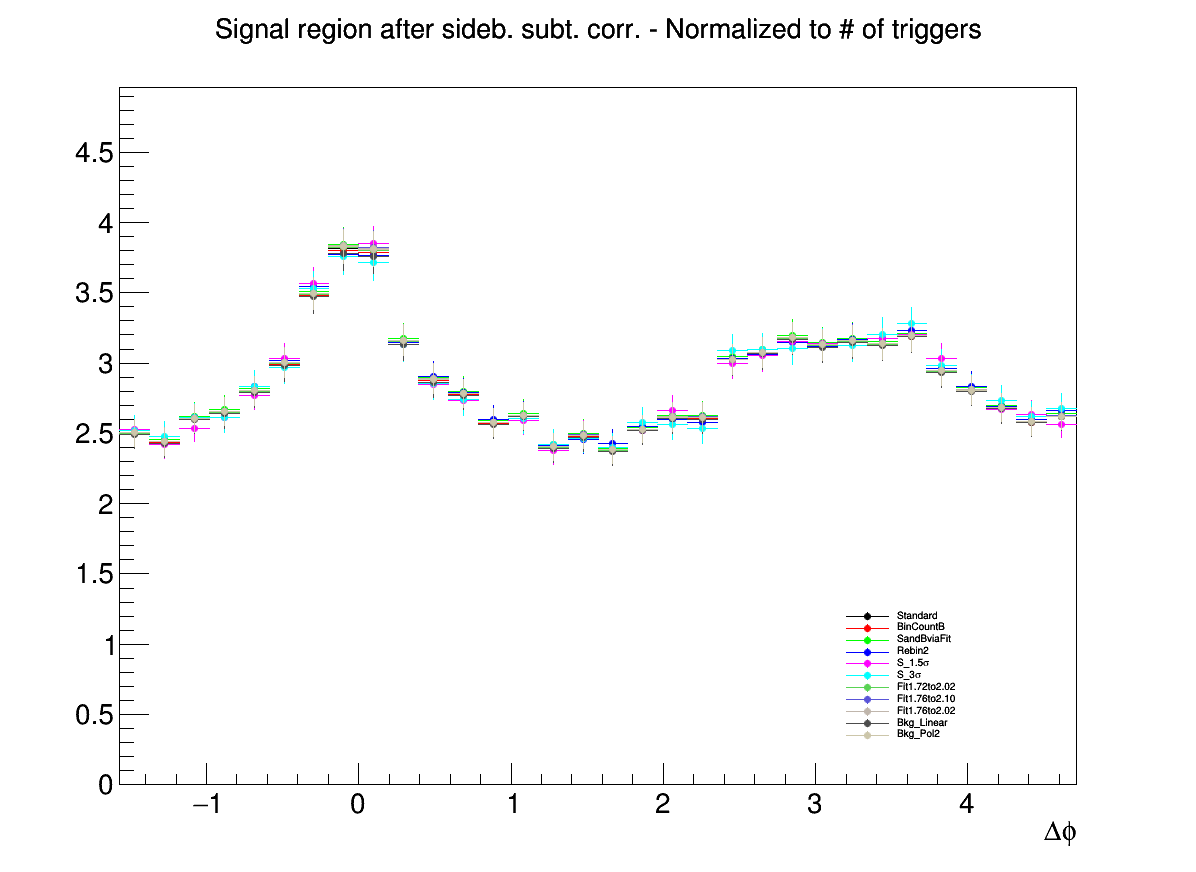
\includegraphics[width=0.47\linewidth, height=5.6cm]{figures/Cut_Optimiz_D0/AzimCorrDistr_Dzero_Canvas_PtIntBins6to8_PoolInt_thr03to99_Superimp.png}}
{\includegraphics[width=0.47\linewidth, height=5.6cm]{figures/Cut_Optimiz_D0/Uncertanty_AzimCorrDistr_Dzero_Canvas_PtIntBins6to8_PoolInt_thr03to99.png}}
{\includegraphics[width=0.47\linewidth, height=5.6cm]{figures/Cut_Optimiz_D0/AzimCorrDistr_Dzero_Canvas_PtIntBins9to10_PoolInt_thr03to99_Superimp.png}}
{\includegraphics[width=0.47\linewidth, height=5.6cm]{figures/Cut_Optimiz_D0/Uncertanty_AzimCorrDistr_Dzero_Canvas_PtIntBins9to10_PoolInt_thr03to99.png}}

\caption{$\Dzero$-h correlation distributions with different cut options (left) and point-by-point relative statistical uncertainty (right) for $3< p_{T}^{\text{D}}< 5$ $\gev/c$ (top), $5< p_{T}^{\text{D}}< 8$ $\gev/c$ (middle), $8< p_{T}^{\text{D}}< 16$ $\gev/c$ (bottom), in all cases with associated track $\pt$ $> 0.3$ $\gev/c$.}
\label{fig:cutoptD0}
\end{figure}

 \subsubsection{Extension to vey-low $\pt$ of D mesons}
 
Thanks to the higher statistic of the 2017 pp data sample, we tried to enlarge our correlation studies to very-low $\pt$ of the trigger particle. Indeed, the figure \ref{fig:VeryLowPt} shows the good performance on the invariant mass extraction for all the 3 D-mesons with $2< p_{T}^{\text{D}}< 3$ $\gev/c$.
\begin{figure}[!htp]
\centering
{\includegraphics[width=1\textwidth]{figures/DplusPlotsweff/InvMassDistributions_Dplus_Bins2to2.png}}
{\includegraphics[width=1\textwidth]{figures/Dzero/InvMassDistributions_Dzero_Bins3to3.png}}
{\includegraphics[width=1\linewidth]{figures/DStar_pp/InvMassDistributions_Dstar_Bins2to3.png}}
\caption{Invariant mass distribution of $\Dplus$ (top), $\Dzero$ (mid) and $\Dstar$ (bottom) corrected with efficiency for  $2< p_{T}^{\text{D}}< 3$.}
\label{fig:VeryLowPt}
\end{figure}

The extension of the analysis to this $\pt$ interval is of high interest in the jet structure characterizion. Indeed, this study allow us to investigate a kinematic region in which the trigger particle has compatible or even lower momentum with respect to the associated particles. This give us the possibility to better understand the production processes. In fact, for example, at the Leading Order (LO) for $\pt (trig) \sim \pt(ass)$ we don't expect any peak on the near-side region. A peak could arise only from Next-to-Leading-Order production process.

Despite the good statistics, it wasn't enough to perform the correlation analysis. Indeed, the correlation distribution suffered of fluctuation expecially on the away-side region where most of the fit failed. 



\subsection{Code used for the analysis}
The code used for D meson-hadron correlation analysis is fully committed in AliPhysics. The analysis classes can be found in
\$ALICE\_ROOT/PWGHF/correlationHF/.  The  D meson specific classes where the aforementioned steps are carried out are
AliAnalysisTaskDStarCorrelations, AliAnalysisTaskSED0Correlations and AliAnalysisTaskDplusCorrelations. The classes which are common to the D meson specific analysis which includes the associated particle cuts and the correlation observables are AliHFAssociatedTrackCuts, AliHFCorrelator, AliHFOfflineCorrelator, AliReducedParticle and AliDhCorrelationExtraction. Several additional classes and macros in the same folder deal with the correction steps.

%The final results presented here are extracted are the HFCJ pPb (n. 88) train runs 290-293 (for $\Dzero$ and $\Dplus$) and 286-289 (for $\Dstar$).

\subsection{Further details on corrections}
\subsubsection{Event Mixing}
%\documentclass[10pt]{article}
%\usepackage[usenames]{color} %usato per il colore
%\usepackage{amssymb} %maths
%\usepackage{amsmath} %maths
%\usepackage[utf8]{inputenc} %utile per scrivere direttamente in caratteri accentuati
%\begin{document}
\label{MEsection}
The event-mixing technique is used for correcting the raw correlation distribution for effects arising
from the detector limited acceptance in rapidity and detector spatial inhomogeneities. The calculation of the Event
Mixing correlation distribution is performed online. %, following the strategy and the code developed for the \textit{PWGCF} correlation analyses.
An event pool is created, where events preceding the one containing a D candidate are stored based on their properties (position of the vertex along the z axis and multiplicity).
Each time a D meson candidate is found in an event, only the events contained in the same pool as the event under analysis is used to evaluate the correlations for the event mixing correction.% the correlation analysis on the mixed events is performed if the pool satisfies the conditions defined at its creation, being the same as described for the pp analysis (As well as the conditions for refreshing the pools).

%For $\Dzero$ and $\Dplus$, an offline approach for the mixed-event correction has been developed. In this approach, D-meson triggers and associated tracks from every analyzed event are stored in dedicated TTree, together with the needed kinematic information to build correlation distributions, and with identifiers of the events to which they belong. In this way, it is possible to correlate each D meson with all the tracks belonging to the same pool over the full event sample, and not being limited to the same subjob as for the online analysis. This allows to increase the statistics of the mixed-event correlation distributions. If was verified that online and offline approaches are fully compatible within the statistical uncertainties.

The multiplicity and z vertex position bins for the pools used in the p-Pb analysis (for both approaches) are the following:
\begin{itemize}
\item Multiplicity bins: $\left(0,20\right);\left(20,35\right);\left(35,+\infty\right)$
\item Vertex z $(cm)$ = $\left(-10,-2.5\right);\left(-2.5,2.5\right);\left(2.5,10\right)$
\end{itemize}
%(\ref{tab:em})

In an ideal case, the mixed event distribution is expected to have a constant flat distribution as function of $\Delta\varphi$ and a triangular shaped distribution in $\Delta\eta$
deriving from the limited $\eta$ acceptance of the detector. In case, instead, of detector inefficient regions, or holes, in the same angular position for D meson and associated tracks, these structures produce an excess of correlations at $\Delta\varphi=0$ in the $\Delta\varphi$ distribution, plus possibly other structures depending on the relative position of the inefficient regions and on their number. The mixed-event distribution is used as a weight in each correlation bin, i.e, the corrected correlation distribution is calculated as follows:
\begin{equation}
\label{eq:mixing}
\frac{dN^{corr}\left(\Delta\varphi \Delta\eta\right)}{d\Delta\varphi d\Delta\eta} = \frac{\frac{dN^{SE}\left(\Delta\varphi \Delta\eta\right)}{d\Delta\varphi d\Delta\eta} }{\frac{dN^{ME}\left(\Delta\varphi \Delta\eta\right)}{d\Delta\varphi d\Delta\eta} }\frac{dN^{ME}\left(0,  0\right)}{d\Delta\varphi d\Delta\eta}
\end{equation}
In Eq.\ref{eq:mixing}, the last term stands for the average of the bins in the region $-0.2 < \Delta\eta < 0.2$, $-0.2 < \Delta\varphi < 0.2$ (multiple bins are used to minimize the effect of statistical fluctuations on the normalization of the mixed-event plots).
This kind of normalization, adopted in the analysis of hadron-hadron correlations, relies on the fact that at $(\Delta\eta,\Delta\varphi)=(0,0)$ the trigger and associated particle experience the same detector effects. In the D meson case this is true only on average and not at very low $\pt$, since D mesons are reconstructed from particles that can go
in different detector region. However, $(\Delta\eta,\Delta\varphi)=(0,0)$ is in any case
the region with maximum efficiency for the pairs (both correlated and uncorrelated). Thus the same convention was adopted.

The mixed-event correlation distributions are built in both D meson signal and sideband regions. Both are
corrected with the relative distributions. An example of the mixed-event distributions, and of the outcome of the mixed-event correction, is provided in Figures \ref{fig:DStarME} and \ref{fig:Dsubtr2D}. The expected triangular shape in $\Delta\eta$, for the mixed-event distributions, addresses the effect of the limited detector pseudo-rapidity acceptance. Note that the mixed-event distribution is limited to the interval $\left|\Delta\eta\right|<1$: the decision to limit the mixed-event correction, and thus the whole analysis, to this range was taken in order to avoid the so-called ``wing effect", i.e. the wing-like structures arising in the correlation distribution at large $\Delta\eta$ due to the limited filling of the correlation bins in that region. %Examples of single-event, mixed-event and ME-corrected correlation distributions, for the same kinematic region of Fig. \ref{fig:DzeroME} but in larger $\left|\Delta\eta\right|$ ranges (1.2, 1.4 and 1.6) are shown in Figs. \ref{fig:DzeroMElarge1}, \ref{fig:DzeroMElarge2} and \ref{fig:DzeroMElarge3}.

\begin{figure}
\centering
{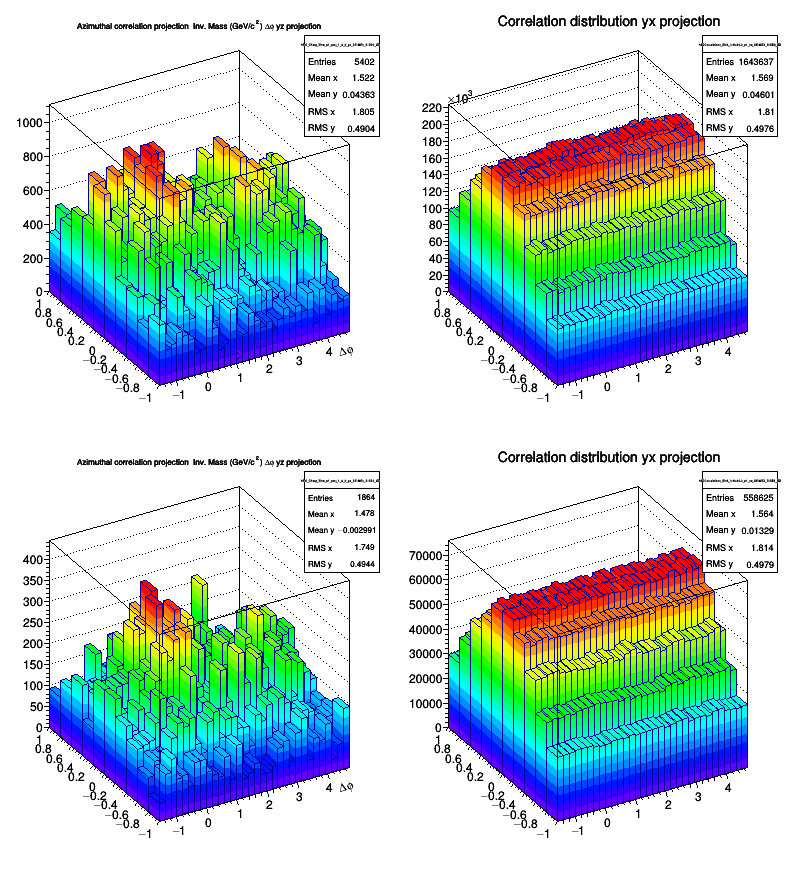
\includegraphics[width=1\linewidth]{figures/Dzero/InputCorr_Dzero_Canvas_pool1_pTbin4_thr03to99.png}}
 \caption{$\Dstar$ meson ($\Delta\varphi$, $ \Delta\eta$) correlation for in the signal region (top row) and sidebands (bottom row) from pool1, for Single Event (left) and Mixed Event analysis (center) for high $p_\mathrm{T}$: $3 < p_\mathrm{T}<5$ GeV/c with associated $p_\mathrm{T} >$ 0.3 GeV/c. The right column shows the SE/ME corrected distributions.}
\label{fig:DStarME}
\end{figure}

\begin{figure}
\centering
{\includegraphics[width=0.9\linewidth, height = 7cm]{figures/Dzero/h2D_Dzero_Subtr_Canvas_PtIntBins9to11_PoolInt_thr1dotto99dot.png}}
\caption{($\Delta\varphi$, $\Delta\eta$) correlation distribution of $D^{*+}$-h with $8 < \pt < 16$ GeV/c and associated track $\pt$ Threshold: $\pt > 0.3$ GeV/c, after the mixed-event correction.}
\label{fig:Dsubtr2D}
\end{figure}
\clearpage
%\end{document}




\begin{comment}
\begin{figure}[!ht]
\centering
%{\includegraphics[width=.95\linewidth]{figures/Dplus_low_dot5_SEbyME.png}}
 \caption{($\Delta \varphi , \Delta \eta$) correlation in the Sidebands and Signal region from Single Event and Mixing Event analysis for low $p_{T}$: $3 < p_{T}^{\text{D}^+} < 5 $\gev/c$$ with associated track $p_{T}$ threshold 0.3 $\gev/c$ }
\label{fig:DplusSEbyMEPlots1}
\end{figure}



\begin{figure}[!ht]
\centering
%Marianna
%{\includegraphics[width=.95\linewidth]{figures/Dplus_mid_dot5_SEbyME.png}}
 \caption{($\Delta \varphi , \Delta \eta$) correlation in the Sidebands and Signal region from Single Event and Mixing Event analysis for mid $p_{T}$: $5< p_{T}^{\text{D}^+}< 8 $\gev/c$$ with associated track $p_{T}$ threshold 0.3 $\gev/c$ }
\label{fig:DplusSEbyMEPlots2}
\end{figure}

\begin{figure}[!ht]
\centering
%{\includegraphics[width=.95\linewidth]{figures/Dplus_high_dot5_SEbyME.png}}
 \caption{($\Delta \varphi , \Delta \eta$) correlation in the Sidebands and Signal region from Single Event and Mixing Event analysis for high $p_{T}$: $8< p_{T}^{\text{D}^+}< 16 $\gev/c$$ with associcated track $p_{T}$ threshold 0.3 $\gev/c$ }
\label{fig:DplusSEbyMEPlots3}
\end{figure}

Figures \ref{fig:DplusSEbyMEPlots1}, \ref{fig:DplusSEbyMEPlots2}, \ref{fig:DplusSEbyMEPlots3} show the 2D correlation in Sideband Region and Signal region from SE and ME analysis for $D^+$ meson in different $p_{T}$ region.

\end{comment}


\newpage
\subsubsection{Tracking and D-meson trigger efficiency}
{\bf \normalsize (i) Tracking efficiency} - The tracking efficiency was calculated by obtaining the ratio between the yield at the reconstructed level and generated level, for a defined ``type" of particles (in our case non-identified particles) and it is estimated differentially in p$_T$, $\eta$, and z$_{vtx}$ of the charged particles.\\

Tracking efficiency maps were produced as TH3D histograms (p$_T$, $\eta$, z$_{vtx}$) obtained from MC analysis on the minimum-bias samples LHC17l3b$\_$fast and LHC17l3b$\_$cent$\_$woSDD anchored to LHC17p,q data samples, considering only primary pions, kaons, protons, electrons and muons, and applying at reconstructed level the track selections (summarized in Table~\ref{table:effCuts}). These efficiency maps were used in the analysis tasks to extract single track efficiencies; each correlation pairs found in the data analysis was inserted in correlation plots with a weight of {\bf 1/efficiency value}.
%As a cross-check, the tracking efficiency was evaluated, with the same criteria, also on the LHC17f2a$\_$fast and LHC17f2a$\_$cent$\_$woSDD samples, which were produced with EPOS-LHC generator instead of DPMJET. Compatibility within 1\% between the efficiency values on the two samples was found.
The 1D ($\pt$ dependence) tracking efficiency for all the five species as well as the tracking efficiency specie by specie are shown in Fig.~\ref{fig:trackeff}.

\begin{figure}[h]
	\centering
	\includegraphics[width=0.55\linewidth, height=0.43\linewidth]{figures/Effs/TrackEff_1D_5Species.png}
    \includegraphics[width=0.4\linewidth]{figures/Effs/TrackEff_1D_e.png}
    \includegraphics[width=0.4\linewidth]{figures/Effs/TrackEff_1D_mu.png}
    \includegraphics[width=0.4\linewidth]{figures/Effs/TrackEff_1D_pi.png}
    \includegraphics[width=0.4\linewidth]{figures/Effs/TrackEff_1D_k.png}
    \includegraphics[width=0.4\linewidth]{figures/Effs/TrackEff_1D_p.png}
	\caption{1D (vs $\pt$) tracking efficiency map for standard track selection, evaluated for five species (electron, muon, pion, kaon and proton) and also different species using data sample LHC17l3b$\_$fast.}
	\label{fig:trackeff}	
\end{figure}

\newpage
Details of cuts at event level and particle/track selection at different steps are listed in Table ~\ref{table:effCuts} . \\
\begin{table}[h]
\small
\centering % used for centering table

\begin{tabular}{  p{5cm} |  p{8.5cm} }
 \\
  \multirow{1}{*}{\large \textbf {MC Generated }} \\
\hline
\\
     Stages         &              Cuts \\
\hline\hline & \\		            	
  1.MC Part with Generated Cuts         &    {\textbf {After Event Selection}}\\
																		   & Charge\\
																		    & PDG Code\\
														  				  & Physical Primary \\

   2. MC Part with Kine Cuts         &              {\textbf {Kinematics Cuts }}\\
															    & -0.8$\textless \eta \textless  0.8$\\
															    & $\pt$ $\textgreater$ 0.3 (GeV/$c$)\\

&		\\            	


\multirow{1}{*}{\large \textbf {MC Reconstructed }} & \\
\hline


\hline & \\		            	                        	
4. Reco tracks        &                             {\textbf {After Event Selection}}\\
															   & Physical Primary \\
															
															
5. Reco tracks with Kine Cuts         &               {\textbf  {Kinematics Cuts }}\\
															    & -0.8$\textless \eta \textless  0.8$\\
															    & $\pt$ $\textgreater$ 0.3 (GeV/$c$)\\



6. MC true with Quality Cuts         &      			      {\textbf  {Quality Cuts }} \\
																	&SetRequireSigmaToVertex(kFALSE) \\
																	&SetDCAToVertex2D(kFALSE) \\
																	&SetMinNCrossedRowsTPC(70)\\
																	&SetMinRatioCrossedRowsOverFindableClustersTPC(0.8)\\
																	&SetMinNClustersITS(2)\\
																	&SetMaxChi2PerClusterTPC(4)\\
																	&SetMaxDCAToVertexZ(1) \\
																	&SetMaxDCAToVertexXY(1) \\
																	&SetRequireTPCRefit(TRUE) \\
																	&SetRequireITSRefit(FALSE) \\

7. Reco tracks with Quality Cuts         &             {\textbf  {Same as step 6}} \\

 &\\		            	            		

 \hline \hline
 \\
\end{tabular}
\caption{\large {The list of event and particle/track selection cuts used in the estimation of single track efficiency}} % title of Table
\label{table:effCuts}	
\end{table}

{\bf \large (ii) D meson efficiency} - Due to limited statistics, the correlation analysis is performed in quite wide $\pt$ bins and in each of them the reconstruction and selection efficiency of D mesons is not flat, in particular in the lower $\pt$ region. We correct for the $\pt$ dependence of the trigger efficiency within each p$_\mathrm{T}$-bin.

This correction is applied online, by using a map of D meson efficiency as a function of $\pt$ and event multiplicity (in terms of SPD tracklets in $|\eta|<1$) extracted from the enriched Monte Carlo sample LHC18a4a2$\_$fast. The $\eta$ dependence was neglected due to the statistics of the available Monte Carlo sample, which rule out the possibility of performing a 3D study.

To properly count the number of trigger particles used to normalize the correlation distributions, $N_\text{trig}$, each D meson is weighted with the inverse of its efficiency in the invariant mass distribution. The main role of the correction for the D meson efficiency is to account for the $\pt$ dependence of the correlation distribution within a given D meson $\pt$ interval. Indeed, only the $\pt$ shape of the D meson efficiency within the correlation $\pt^{\rm trig}$ ranges is relevant while the average value
in the $\pt$ range is simplified due to the normalization of the correlation distribution to the number of trigger particles.

Efficiency plots for $\Dzero$, $\Dplus$ and $\Dstar$ mesons are shown in Figs.~\ref{fig:dEffPrompt} and ~\ref{fig:dEffFD}, for prompt and feed-down D mesons, respectively.

\begin{figure}[!htp]     %da c
	\centering
%Marianna
    \includegraphics[width=.48\linewidth]{figures/Effs/EfficiencyMap_2D_DPlus_c_Ref_wLimAcc_Plot.png}
	\includegraphics[width=.48\linewidth]{figures/Effs/EfficiencyMap_1D_DPlus_c_Ref_wLimAcc_Plot.png}  % by Fabio
	\includegraphics[width=.48\linewidth]{figures/DStar_pp/EfficiencyMap_2D_DStar_c_final_wLimAcc_Plot.png}
	\includegraphics[width=.48\linewidth]{figures/DStar_pp/EfficiencyMap_1D_DStar_c_final_wLimAcc_Plot.png}  % by Fabio
	\includegraphics[width=.48\linewidth]{figures/Effs/EfficiencyMap_2D_Dzero_c_RefPtBins_wLimAcc_Plot.png}
	\includegraphics[width=.48\linewidth]{figures/Effs/EfficiencyMap_1D_Dzero_c_RefPtBins_wLimAcc_Plot.png}  % by Fabio
	
	%\includegraphics[width=.30\linewidth]{figures/D0Eff_ProjMult_3to4GeV.png}
	%\includegraphics[width=.30\linewidth]{figures/D0Eff_ProjMult_5to6GeV.png}
	%\includegraphics[width=.30\linewidth]{figures/D0Eff_ProjMult_8to12GeV.png}
\caption{Top panel: ($\pt$, multiplicity) dependence (left) and $\pt$  dependence (right) of prompt $\Dplus$ meson efficiency.
Mid panel: ($\pt$, multiplicity) dependence (left) and $\pt$  dependence (right) of prompt $\Dstar$ meson efficiency.
Bottom panel: ($\pt$, multiplicity) dependence (left) and $\pt$  dependence (right) of prompt $\Dzero$ meson efficiency.
%s: multiplicity dependence of $D^0$ meson efficiency for three $D^0$ p$_\mathrm{T}$ ranges: 3-4 GeV/$c$ (left), 5-6 GeV/$c$ (center), 8-12 GeV/$c$ (right). For tracklet multiplicity$>$ 120, due to the limited statistics, the efficiency value is fixed to the one obtained for 90$<$tracklet multiplicity$<$120.
}
	\label{fig:dEffPrompt}	
\end{figure}

\begin{figure}[h]   %da B
	\centering
	%Marianna
		  % by Fabio
	\includegraphics[width=.48\linewidth]{figures/Effs/EfficiencyMap_2D_DPlus_b_Ref_wLimAcc_Plot.png}
	\includegraphics[width=.48\linewidth]{figures/Effs/EfficiencyMap_1D_DPlus_b_Ref_wLimAcc_Plot.png}
	  % by Fabio
	\includegraphics[width=.48\linewidth]{figures/DStar_pp/EfficiencyMap_2D_DStar_b_final_wLimAcc_Plot.png}
	\includegraphics[width=.48\linewidth]{figures/DStar_pp/EfficiencyMap_1D_DStar_b_final_wLimAcc_Plot.png}
	  % by Fabio
	\includegraphics[width=.48\linewidth]{figures/Effs/EfficiencyMap_2D_Dzero_b_RefPtBins_wLimAcc_Plot.png}
	\includegraphics[width=.48\linewidth]{figures/Effs/EfficiencyMap_1D_Dzero_b_RefPtBins_wLimAcc_Plot.png}
	\caption{Top panel: ($\pt$, multiplicity) dependence (left) and $\pt$ dependence (right) of feed-down $\Dplus$ meson efficiency.
Mid panel: ($\pt$, multiplicity) dependence (left) and $\pt$ dependence (right) of feed-down $\Dstar$ meson efficiency.
Bottom panel: ($\pt$, multiplicity) dependence (left) and $\pt$ dependence (right) of feed-down $\Dzero$ meson efficiency.}
	\label{fig:dEffFD}	
\end{figure}
\clearpage

%It was observed that multiplicity dependence of the efficiency does not bias the extraction of the signal yield from the invariant mass distributions (which, as anticipated, are also weighted in the same manner). In addition, the multiplicity dependence of the efficiencies (shown for the $\Dzero$, in integrated $\pt$ range, in Fig. \ref{fig:DeffY}) is rather flat in the range 20-80 tracklets, where about 90\% of the reconstructed D-mesons are found, which explains why it has a negligible effect on the correlation distributions on this data sample.
%\begin{figure}[h]   %da B
%	\centering
%	\includegraphics[width=.48\linewidth]{figures/Effs/EfficiencyMap_1D_Dzero_c_RefPtBins_Ydep_wLimAcc_Plot.png}
%\caption{Prompt $\Dzero$ meson efficiency as a function of multiplicity (SPD tracklet in $|\eta|<1$).}
%	\label{fig:DeffY}	
%\end{figure}
\clearpage


\subsubsection{Correction for bias on B to D decay topologies}
\label{MCclosure}
To verify the consistency of the analysis chain and of the corrections applied to the  correlation distributions extracted from data, a Monte Carlo closure test was setup and tried on the $\Dzero$-h analysis.

On the Monte Carlo enriched with charm and beauty quarks (LHC18a4a2$\_$fast, with GEANT3), the correlation analysis was performed both at kinematic level and at reconstructed level. At kinematic level, only acceptance cuts were applied on the D mesons and the associated particles, using the Monte Carlo information for the identification of the D mesons and the hadrons in the event and rejecting the non-primary particles. At reconstructed level, the analysis was performed as if it were executed on data, applying the event selection, the acceptance cuts for D mesons and the associated particles, selecting the D meson candidates with filtering cuts on their daughters, topological cuts and PID selection, and then keeping only the true D mesons by matching with the Monte Carlo truth; non-primary particles were rejected by means of the DCA selection. Event mixing correction was applied both at reconstructed and at kinematic level, where it takes into account just the effects of the acceptance cuts. In addition, at reconstructed level, the efficiency corrections for D mesons and associated tracks were also applied.

The consistency check was performed to verify whether, after having applied all the corrections to the azimuthal correlation plots at reconstructed level, the results were compatible with the ones at kinematic level. Hence, the ratios of fully corrected reconstructed plots over kinematic plots were evaluated in all the $\Dzero$ $p_\text{T}$ bins and for the various $p_\text{T}$ thresholds for the associated tracks, separating the contributions for the different origins of particles and triggers. The ratios, shown in Figure~\ref{fig:MC_Ratios} for exemplary kinematic regions (covering anyway the full span of the measurement), denote a good compatibility with 1, within the uncertainties, of the average reconstructed over generated ratios, in particular for the all D-non HF track case (blue curves), apart from small downward deviations at low $\pt$, which will be cured with a 2-3\% asymmetric systematic uncertainty, as also previously done in the pp 2010 and p--Pnb 2013 analyses.

The major exceptions to the previous conclusion are clearly the structures in the near side region for the beauty origin case.
It was verified that these structures are induced by our topological selection for the D mesons. Indeed, in cases in which the D meson triggers come from B hadrons, applying the topological cuts (especially the cosine of the pointing angle) tends to favour cases with a small angular opening between the products of the B hadron decay (i.e. the D meson trigger itself and other particles), with respect to cases where the B decay particles are less collinear.

\begin{figure}
\centering
{\includegraphics[width=.48\linewidth]{figures/MC_closure/MCClosure_Dzero_Canvas_PtIntBins4to5_PoolInt_thr03to1.png}}
{\includegraphics[width=.48\linewidth]{figures/MC_closure/MCClosure_Dzero_Canvas_PtIntBins4to5_PoolInt_thr1to99.png}} \\

{\includegraphics[width=.48\linewidth]{figures/MC_closure/MCClosure_Dzero_Canvas_PtIntBins6to8_PoolInt_thr03to1.png}}
{\includegraphics[width=.48\linewidth]{figures/MC_closure/MCClosure_Dzero_Canvas_PtIntBins6to8_PoolInt_thr1to99.png}} \\

{\includegraphics[width=.48\linewidth]{figures/MC_closure/MCClosure_Dzero_Canvas_PtIntBins9to11_PoolInt_thr03to1.png}}
{\includegraphics[width=.48\linewidth]{figures/MC_closure/MCClosure_Dzero_Canvas_PtIntBins9to11_PoolInt_thr1to99.png}} \\

{\includegraphics[width=.48\linewidth]{figures/MC_closure/MCClosure_Dzero_Canvas_PtIntBins12to13_PoolInt_thr03to1.png}}
{\includegraphics[width=.48\linewidth]{figures/MC_closure/MCClosure_Dzero_Canvas_PtIntBins12to13_PoolInt_thr1to99.png}}
\end{figure}
\begin{figure}
\centering
\caption{Ratios of fully corrected azimuthal correlation plots at reconstructed level over azimuthal correlation plots at kinematic level, in the two $\Dzero$ $p_\text{T}$ bins, for the different associated $p_\text{T}$ ranges. Black points: All $\Dzero$-all hadrons, normalized by all $\Dzero$ triggers; light red points: $\Dzero$ from c-hadrons from c, normalized by c-$\Dzero$ triggers; dark red points: $\Dzero$ from c-all hadrons, normalized by c-$\Dzero$ triggers; light green points: $\Dzero$ from b-hadrons from b, normalized by b-$\Dzero$ triggers; dark green points: $\Dzero$ from b-all hadrons, normalized by b-$\Dzero$ triggers; blue points: All $\Dzero$-hadrons from light quarks, normalized by all $\Dzero$ triggers.
The panels show the ranges: $3 < \pt$(D)$ < 5$ $\gev/c$ , $0.3 < \pt$(assoc)$ < 1$ $\gev/c$  (1st row-left); $3 < \pt$(D)$ < 5$ $\gev/c$ , $\pt$(assoc)$ > 1$ $\gev/c$  (1st row-right); $5 < \pt$(D)$ < 8$ $\gev/c$ , $0.3 < \pt$(assoc)$ < 1$ $\gev/c$  (2nd row-left); $5 < \pt$(D)$ < 8$ $\gev/c$ , $\pt$(assoc)$ > 1$ $\gev/c$  (2nd row-right);  $8 < \pt$(D)$ < 16$ $\gev/c$ , $0.3 < \pt$(assoc)$ < 1$ $\gev/c$  (3rd row-left), $8 < \pt$(D)$ < 16$ $\gev/c$ , $\pt$(assoc)$ > 1$ $\gev/c$  (3rd row-right); $16 < \pt$(D)$ < 24$ $\gev/c$ , $0.3 < \pt$(assoc)$ < 1$ $\gev/c$  (4th row-left), $16 < \pt$(D)$ < 24$ $\gev/c$ , $\pt$(assoc)$ > 1$ $\gev/c$  (4th row-right).}
\label{fig:MC_Ratios}
\end{figure}

In the Monte Carlo closure test, this situation is reflected in the correlation distributions at reconstructed level, where the topological selection is applied, while it does not occur at kinematic level. Hence, in the reconstructed/kinematic ratio, the distribution would show an excess for $\Delta\varphi = 0$ (due to the favoured decays with small opening angle), which is then compensated by a depletion for larger values of $\Delta\varphi = 0$ (corresponding to B decays with larger angles, which are disfavoured).
These structures are prominent at low $\Dzero$ $p_\text{T}$, where the topological cuts are tighter, and tend to disappear at higher $\pt$, where the selections are released. They are also larger in the higher associated track $\pt$ ranges, where the fraction of B-hadron decay tracks dominate the overall correlation distributions.

The data correlation distribution need to be corrected for this bias, and in particular for the enhancement of b-origin correlation pairs at the centre of the near side region, which would influence the near-side peak features.
In order to do this, the amount of the b-origin excess is evaluated from the Reco/Kine ratio, by considering the b-$\Dzero$-all tracks case (dark green points). The excess at Reco level (affecting data) is quantified as a $\Delta\varphi$ modulation {\bf modul} for the five points an each side of the $\Delta\varphi = 0$ value (or, equivalently, on the first five points of the reflected distributions, which start from $\Delta\varphi=0$. This is done separately in each $\pt$ range.
Then, the correction is done by applying this modulation to the data correlation distributions, but taking into account that only the correlation entries from B$\rightarrow$D are affected, while the c$\rightarrow$D correlations need to be left unaltered.
In particular, it has to be considered that:
\begin{itemize}
\item On data, the B$\rightarrow$D correlation pairs are only a fraction (1-$\fprompt$) of the total.
\item The amplitude of B$\rightarrow$D$|_{\rm amplit}$ correlation pattern is different (greater) than the amplitude of the c$\rightarrow$D$|_{\rm amplit}$ correlation pattern:
\end{itemize}

Thus, the following equation is applied to get the corrected $C(\Delta\varphi)_{\rm corr}$ data points starting from the raw ones, $C(\Delta\varphi)_{\rm raw}$:
\begin{equation}
C(\Delta\varphi)_{\rm corr} = C(\Delta\varphi)_{\rm raw} \cdot [\frac{{\rm c}\rightarrow{\rm D}|_{\rm amplit}}{{\rm (B+c)}\rightarrow{\rm D}|_{\rm amplit}} \cdot f_{\rm prompt} + \frac{{\rm B}\rightarrow{\rm D}|_{\rm amplit}}{{\rm (B+c)}\rightarrow{\rm D}|_{\rm amplit}} \cdot (1-f_{\rm prompt})\cdot\frac{1}{\bf modul}]
\end{equation}
where ${\rm (B+c)}\rightarrow{\rm D}|_{\rm amplit} = {\rm c}\rightarrow{\rm D}|_{\rm amplit} \cdot f_{\rm prompt} + {\rm B}\rightarrow{\rm D}|_{\rm amplit} \cdot (1-f_{\rm prompt})$, and where the two amplitudes are evaluated from the Monte Carlo distributions at reconstructed level (so, including the bias), and $\fprompt$ with the procedure described in \ref{BeautyFeedDownSection}.
Applying the {\bf modul} factor to the beauty part of the data correlation distributions brings its value back to the generated level case, effectively removing the bias.
The effect of the correction is a shift of the data points in the near-side region (in general, downward in the first and second points, the upward in the others). The maximum value of the shift is of about 5\%, at the centre of the near-side peak, for the lowest D-meson $\pt$ range ($3 < \pt < 5$ $\gev/c$ ) and the highest associated track $\pt$ range ($\pt > 3$ $\gev/c$ ). The typical values are instead of a couple of percentage points. The correction is zero in the highest D-meson $\pt$ range.
To take into account for possible inaccuracies in the definition of the modulations, or in their rescaling, a systematic uncertainty is  applied on the corrected data points, with value $|C(\Delta\varphi)_{\rm corr} - C(\Delta\varphi)_{\rm raw}|/\sqrt(12)$, on each side of the data points affected by the bias (symmetric uncertainty).

\clearpage
%\end{document}


\subsubsection{Secondary track contamination}
\label{secondaries}
The secondary tracks inside the associated track sample, due to interaction of primary track with the detector material or to decays of strange hadrons, are mostly removed by the DCA cuts applied during the cut selection phase (DCA($xy$) $<$ 1 cm, DCA($z$) $<$ 1 cm).
Anyway, a small fraction of secondary tracks survives this cut, and the data correlation distributions have to be corrected for this residual contamination.
The fraction of surviving secondary tracks is evaluated via a study on the LHC18a4a2$\_$fast sample, by counting the number of tracks accepted by the selection whose corresponding generated-level track doesn't satisfy the IsPhysicalPrimary() call, and dividing this number by the total number of accepted tracks.
The outcome of the check is reported in Figure \ref{fig:secnumber}. As it's visible, no more than 5\% secondary tracks pass the selection. Moreover, the fraction of residual secondary tracks is flat along the $\Delta\varphi$ axis, as shown, for exemplary $\pt$ regions, in Figure \ref{fig:secdPhi}, where the inhomogeneities are always below 1\%.
For this reason, it is possible to directly scale the data correlation distributions by their purity fraction (i.e. 1 - secondary contamination). This is done with an associated $\pt$ dependence, due to the increase of the purity with the track $\pt$, while the purity fraction is taken flat versus the D-meson $\pt$.
The purity values that were choosen are the following (NOT FINAL):
\begin{itemize}
  \item $\pt$(assoc) $> 0.3$ $\gev/c$ : 0.958
  \item $\pt$(assoc) $> 1$ $\gev/c$ : 0.973
  \item $0.3 < \pt$(assoc) $< 1$ $\gev/c$ : 0.953
  \item $1 < \pt$(assoc) $< 2$ $\gev/c$ : 0.969
  \item $2 < \pt$(assoc) $< 3$ $\gev/c$ : 0.982
  %\item $\pt$(assoc) $> 3$ $\gev/c$ : 0.990
\end{itemize}


\begin{figure}[h]   %da B
	\centering
	%Marianna
		  % by Fabio
	\includegraphics[width=.48\linewidth]{figures/SecTracks/FractOfSecOverTotal_2to3.png}
	\includegraphics[width=.48\linewidth]{figures/SecTracks/FractOfSecOverTotal_3to5.png}
	\includegraphics[width=.48\linewidth]{figures/SecTracks/FractOfSecOverTotal_5to8.png}
    \includegraphics[width=.48\linewidth]{figures/SecTracks/FractOfSecOverTotal_8to16.png}
    \includegraphics[width=.48\linewidth]{figures/SecTracks/FractOfSecOverTotal_16to24.png}
	\caption{Fraction of secondary tracks over total amount of tracks which pass the DCA selection. The four panel show the fractions for the D-meson $\pt$ ranges: 2-3, 3-5, 5-8, 8-16, 16-24, respectively. Inside each panel, the associated track $\pt$ ranges are shown on the $x$-axis.}
	\label{fig:secnumber}	
\end{figure}

\begin{figure}[h]   %da B
	\centering
	%Marianna
		  % by Fabio
{\includegraphics[width=0.4\linewidth]{figures/SecTracks/DeltaPhi_2to3_03to1_RatioPrimOverAll.png}}
{\includegraphics[width=0.4\linewidth]{figures/SecTracks/DeltaPhi_2to3_1to99_RatioPrimOverAll.png}}
{\includegraphics[width=0.4\linewidth]{figures/SecTracks/DeltaPhi_3to5_03to1_RatioPrimOverAll.png}}
{\includegraphics[width=0.4\linewidth]{figures/SecTracks/DeltaPhi_3to5_1to99_RatioPrimOverAll.png}} 
{\includegraphics[width=0.4\linewidth]{figures/SecTracks/DeltaPhi_5to8_03to1_RatioPrimOverAll.png}}
{\includegraphics[width=0.4\linewidth]{figures/SecTracks/DeltaPhi_5to8_1to99_RatioPrimOverAll.png}} 
{\includegraphics[width=0.4\linewidth]{figures/SecTracks/DeltaPhi_8to16_03to1_RatioPrimOverAll.png}}
{\includegraphics[width=0.4\linewidth]{figures/SecTracks/DeltaPhi_8to16_1to99_RatioPrimOverAll.png}}
	\caption{Fraction of primary track in the reconstructed associated track sample (blue histogram). The polynomial fit function (red curve) and the 3-point moving average (red histogram) are also superimposed. The $\pt$(D) ranges are 2-3, 3-5, 5-8, 8-16 GeV/$c$, respectively for each row, and $0.3 < \pt$(assoc)$ < 1$, $\pt$(assoc) $> 1$ GeV/$c$ inside each row.}
	\label{fig:secdPhi}	
\end{figure}

It was also verified with the same Monte Carlo study that applying the DCA selection rejects less than 0.2\% primary tracks (tagged as false positives) from the associated track sample, again with a flat azimuthal distribution, inducing hence a fully negligible bias on the data correlation distributions. This is shown in Figure \ref{fig:primRej}. This was also verified for specific charm-origin and beauty-origin tracks, due to their larger DCA with respect to primary tracks from light quarks. In this case, the fraction of rejected charm and beauty tracks stays below 1\% in all the kinematic ranges apart from the associated track $\pt$ regions 0.3-1 and $>0.3$ $\gev/c$ , where the rejection can be as high as 2\%. In these kinematic ranges, though, the data correlation distributions are dominated by non-heavy-flavour tracks, as it was verified from the simulations, hence the overall bias is still contained below 1\%, thus negligible.

\begin{figure}[h]   %da B
	\centering
			  % by Fabio
	\includegraphics[width=.48\linewidth]{figures/SecTracks/FractOfPrimAccepted_2to3.png}
	\includegraphics[width=.48\linewidth]{figures/SecTracks/FractOfPrimAccepted_3to5.png}
	\includegraphics[width=.48\linewidth]{figures/SecTracks/FractOfPrimAccepted_5to8.png}
    \includegraphics[width=.48\linewidth]{figures/SecTracks/FractOfPrimAccepted_8to16.png}
    \includegraphics[width=.48\linewidth]{figures/SecTracks/FractOfPrimAccepted_16to24.png}
	\caption{Fraction of primary tracks rejected by the DCA selection. The four panel show the fractions for the D-meson $\pt$ ranges:2-3, 3-5, 5-8, 8-16, 16-24, respectively. Inside each panel, the associated track $\pt$ ranges are shown on the $x$-axis.}
		\label{fig:primRej}	
\end{figure}

These studies were performed on an enriched Monte Carlo sample, which could not fully reproduce the relative abundancies of the species. Anyway, for events with a reconstructed D-meson, this bias is expected to be minor, and only these events are used in the data analysis. In any case, the percentages obtained from the study were found to be consistent within 1\%.

\clearpage
%\end{document}


\subsubsection{Beauty feed-down}
\label{BeautyFeedDownSection}
The contribution of correlations of D meson from b-hadron decay is subtracted from the data correlation distributions as:
\begin{equation}
\tilde{C}_{\rm prompt~D}(\Delta\varphi)=\frac{1}{f_{\rm prompt}}\left(\tilde{C}_{\rm inclusive}(\Delta\varphi)-(1-f_{\rm prompt})\tilde{C}_{\rm feed-down}^{\rm MC~templ}(\Delta\varphi) \right).
\label{eqFeedDown}
\end{equation}
In the above equation, $\tilde{C}_{\rm inclusive}(\Delta\varphi)$ and $\tilde{C}_{\rm prompt~D}(\Delta\varphi)$ are per-trigger azimuthal correlation distributions before and after
feed-down contribution subtraction, $f_{\rm prompt}$ is the fraction of prompt D meson and $\tilde{C}_{\rm feed-down}^{\rm MC~templ}$ is a template
of the azimuthal correlation distribution for the feed-down component obtained from home-made Monte Carlo simulation at generated level, using PYTHIA6 with Perugia2011 tune.
In order to avoid biases related to the different event multiplicity in real and simulated events, the correlation distribution was shifted to have its minimum coinciding with the baseline of the data azimuthal-correlation distribution before feed-down subtraction. %[THIS HELD FOR pp...]A difference smaller than 8\% was observed in the simulation between the baseline values of the azimuthal-correlation distributions for prompt and feed-down D mesons. Considering the typical values of $f_{\rm prompt}$, this difference results in a shift of the baseline of $\tilde{C}_{\rm prompt~D}(\Delta\varphi$ of less than 1\%, negligible with respect to the other uncertainties affecting the measurement.

The value of $f_{\rm prompt}$ (Figure \ref{fprompt}), which depends on D-meson species and varies as a function of the $\pt$, is estimated on the basis of FONLL predictions for the production of feed-down D mesons at central rapidity, in pp collisions at $\sqrt(s) = 5$ TeV, and using the reconstruction efficiency of prompt and feed-down D mesons, following the so-called $N_{\rm b}$ approach defined in~\cite{ALICEDmespp7Tev}. Typical values are about 8-10\% for the
$\Dzero$, about 4-7\% for the $\Dplus$ and about 5-8\% for the $\Dstar$. %The procedure adopted is the same as what done in the past analysis \cite{Notepp}: however, in p--Pb, in order to consider a possible non-zero $v_{2}$-like modulation of the baseline, a range of $0<v_{2}<0.2$ values for tracks and for secondary D mesons is considered for the systematic uncertainty evaluation (using an hypothesis of no modulation for both cases for central values).
\begin{comment}
\begin{figure}
\centering
\includegraphics[width=0.6\linewidth]{figures/Effs/fprompt_D0.png}
\includegraphics[width=0.6\linewidth]{figures/DStar_pp/Fprompt_Dstar.pdf}
\includegraphics[width=0.6\linewidth]{figures/Effs/fpromptDplus.png}
\caption{$f_{\rm prompt}$ as a function of the $\pt$ for $\Dzero$ (top), $\Dstar$ (mid) and $\Dplus$ (bottom) estimated on the basis of FONLL predictions}
\label{fprompt}
\end{figure}

Examples of the PYTHIA templates used for the feed-down contribution subtraciton are shown in Figures \ref{templates1} (Figure \ref{templates2} shows the same templates but for prompt D mesons).

\begin{figure}
\centering
\includegraphics[width=1\linewidth]{figures/Template/1DCompare_allDpTfromB_AssoPt_0dot3to99dot0GeVc_Perugia2010.png}
\includegraphics[width=1\linewidth]{figures/Template/1DCompare_allDpTfromB_AssoPt_0dot3to99dot0GeVc_Perugia2011.png}
\includegraphics[width=1\linewidth]{figures/Template/1DCompare_allDpTfromB_AssoPt_0dot3to99dot0GeVc_Pythia8.png}
\caption{Azimuthal correlation distribution between D meson from b-hadron decay and charged particles obtained from Monte Carlo simulations
based on Pythia-Perugia2010 tune (row1), Pythia-Perugia2011 tune (row2), Pythia8 tune 4C (row3) for associated track $\pt > 0.3$ $\gev/c$  and D-meson $\pt$ ranges: 3-5, 5-8, 8-16, 16-24 $\gev/c$ . $\Dzero$ in blue, $\Dplus$ in green, $\Dstar$ in red.}
\label{templates1}
\end{figure}

\begin{figure}
\centering
\includegraphics[width=1\linewidth]{figures/Template/1DCompare_allDpTfromC_AssoPt_0dot3to99dot0GeVc_Perugia2010.png}
\includegraphics[width=1\linewidth]{figures/Template/1DCompare_allDpTfromC_AssoPt_0dot3to99dot0GeVc_Perugia2011.png}
\includegraphics[width=1\linewidth]{figures/Template/1DCompare_allDpTfromC_AssoPt_0dot3to99dot0GeVc_Pythia8.png}
\caption{Azimuthal correlation distribution between prompt D meson and charged particles obtained from Monte Carlo simulations
based on Pythia-Perugia2010 tune (row1), Pythia-Perugia2011 tune (row2), Pythia8 tune 4C (row3) for associated track $\pt > 0.3$ $\gev/c$  and D-meson $\pt$ ranges: 3-5, 5-8, 8-16, 16-24 $\gev/c$ . $\Dzero$ in blue, $\Dplus$ in green, $\Dstar$ in red.}
\label{templates2}
\end{figure}

The feed-down subtraction was performed after rescaling the data correlation distributions for the purity fraction, and correcting them by the near-side modulation induced by the bias on the B decay topology.
 \end{comment}
\clearpage

\newpage % always start next (sub)section with new page to avoid disarrangement.


 
